\section{Architecture globale}
    \label{sec:archiGlobale}
    
    \subsection{Prototype d'interface}
    \label{sec:interface}
    
    Voici un prototype de l'interface.
    \begin{figure}[h!]
        \centering
        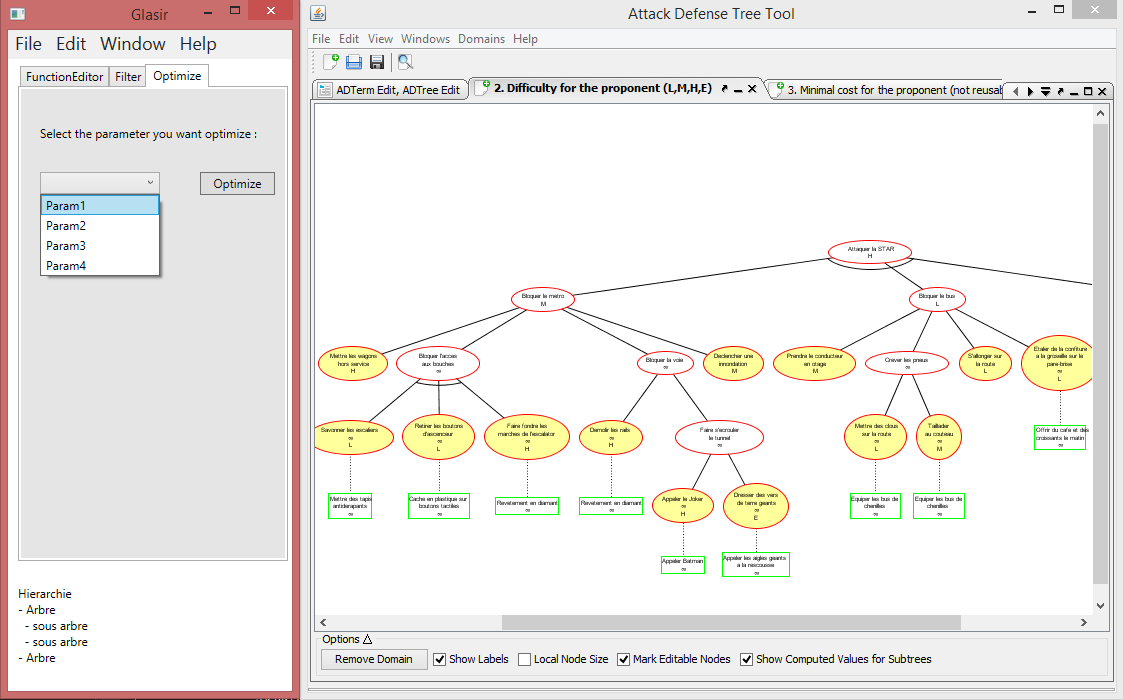
\includegraphics[height=0.4\textwidth]{figure/interface.png}
        \caption{Prototype de l'interface de \glasir{}.}
        \label{fig:glasir}
    \end{figure}
    
    Les fonctions filtre et tout seront facilement accessibles. On aura adtool au milieu ou pas, blablabla.
    
    \subsection{Diagramme de cas d'utilisation}
    \label{sec:casutil}
    	Ce diagramme décrit les cas d'utilisation, voilà.

    \begin{figure}[H]
        \centering
        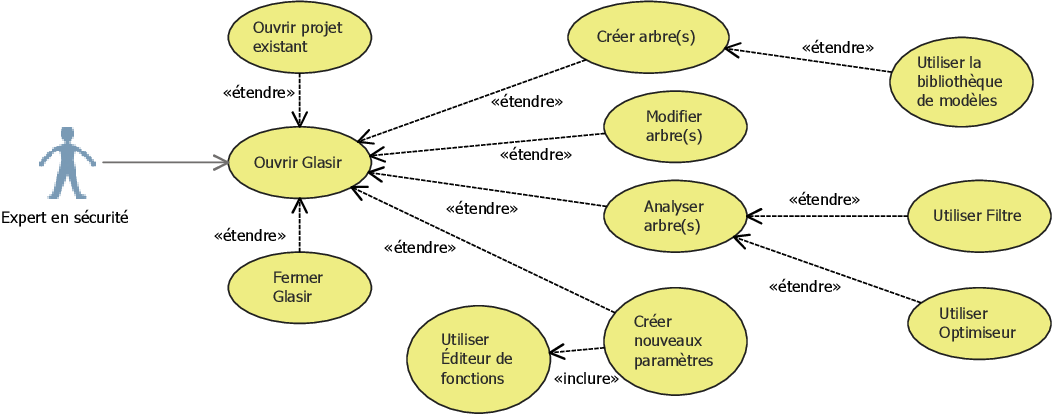
\includegraphics[height=0.5\textwidth]{figure/UseCaseDiagram.png}
        \caption{Diagramme de cas d'utilisation de Glasir.}
        \label{fig:use_case}
    \end{figure}
    